% L10a lecture companion. Notebook hashes and coverage are recorded in README.md.
% Style files and Cornell seal are copied unchanged from the L9a deck (identical
% to L7c, L7a, and L6c, which match the approved L6a deck). The agent-environment
% schematic is converted from ../figs/Fig-Schematic-RL.svg to a light PDF, and
% the weighted majority figure is the light PDF from ../figs/Fig-WMA-Weights,
% both copied into assets/ by `make figures`.
%
% Notation follows the lecture: experts i = 1, ..., n, rounds t = 1, ..., T,
% weights w_i^{(t)}, the WMA learning rate epsilon, the MWA learning rate eta,
% the distribution p^{(t)}, signed costs m_i^{(t)}, mistakes M^{(t)} and
% M_i^{(t)}, and the regret R(T).
\documentclass[aspectratio=169,11pt]{beamer}
\usepackage{vnslides}
\renewcommand{\vnlecturecode}{L10a}
\newcommand{\lecturelink}{https://github.com/varnerlab/CHEME-5800-CourseRepository-Fall-2026/blob/main/weeks/week-10/L10a/CHEME-5800-L10a-Lecture-OnlineLearningAndRegret-Fall-2026.ipynb}
\newcommand{\lablink}{https://github.com/varnerlab/CHEME-5800-CourseRepository-Fall-2026/blob/main/weeks/week-10/L10b/CHEME-5800-L10b-Lab-WeightedMajorityAlgorithm-Fall-2026.ipynb}
\newcommand{\lecturesource}[1]{\note{[Sources]\par
  \href{\lecturelink}{L10a lecture: Online Learning: Weighted Majority and Multiplicative Weights Algorithms.}\par
  #1\par[/Sources]}}
\newcommand{\pv}{\mathbf p}
\newcommand{\mv}{\mathbf m}

\title{\texorpdfstring{{\vnheavy L10a}}{L10a}: Online Learning}
\subtitle{\texorpdfstring{Regret, weighted majority, and multiplicative weights\\[3pt]CHEME 5800 Cornell University}{Regret, weighted majority, and multiplicative weights; CHEME 5800 Cornell University}}
\author{Copyright Jeffrey Varner 2026. All Rights Reserved}

\begin{document}
\special{pdf:minorversion 7}
\vntitlepage

\begin{frame}{Objectives for Today}
  How can we learn from a sequence of outcomes chosen by an adversary, and how
  do we judge how well we learned?

  \vspace{0.4em}
  {\large\textbf{\ink{Today's concepts}}}
  \vspace{0.2em}
  \begin{itemize}\setlength{\itemsep}{0.4em}
    \item \hilite{Describe the online learning problem}: a game over many
      rounds; we predict, an adversary reveals the outcome, and we learn from
      the result.
    \item \hilite{Measure an online learning algorithm with regret}: compare
      its loss with the best fixed strategy in hindsight, and seek a regret
      bound that grows more slowly than the number of rounds.
    \item \hilite{Learn from expert advice with multiplicative weights}: shrink
      the weight of each expert that does poorly, and bound how far we fall
      behind the best expert.
  \end{itemize}
  \slidenote{Lecture:}{\href{\lecturelink}{Online Learning: Weighted Majority and Multiplicative Weights}}
  \lecturesource{Introduction and three Learning Objectives.}
\end{frame}

\begin{frame}{The Reinforcement and Online Learning Problem}
  An agent observes a state $s$ from its set of states $\mathcal S$, takes an
  action $a$ from its set of actions $\mathcal A$, and receives a reward $r$. How does it learn to choose actions that maximize
  its cumulative reward?

  \vspace{0.2em}
  \centering
  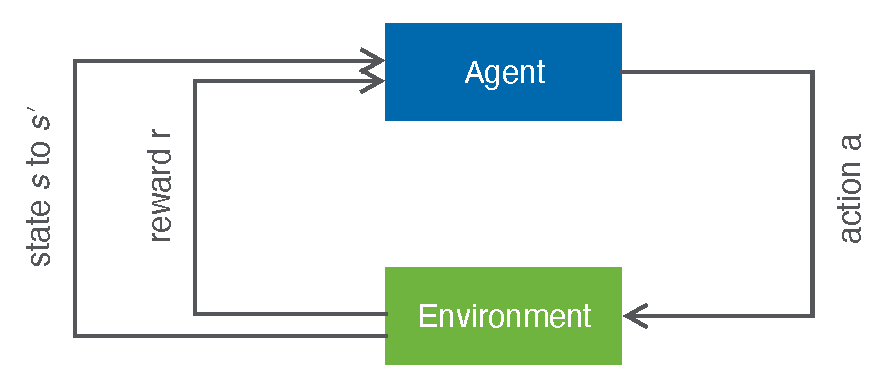
\includegraphics[width=\textwidth,height=0.47\paperheight,keepaspectratio]{assets/Fig-Schematic-RL.pdf}

  \vspace{0.2em}
  \raggedright
  The agent selects an action, receives a reward, and moves from state $s$ to
  the next state $s'$. The reward shapes its future decisions.
  \lecturesource{General Reinforcement/Online Learning Problem: opening paragraph and figure.
    Figure: ../figs/Fig-Schematic-RL.svg, converted to a light PDF with rsvg-convert.}
\end{frame}

\begin{frame}{Three Families of Methods}
  \begin{itemize}\setlength{\itemsep}{0.7em}
    \item \hilite{Multiplicative weights} update expert weights based on their
      past performance.
    \item \hilite{Bandit algorithms} observe only the reward of the action
      they take; in the basic multi-armed bandit, there is no evolving state.
    \item \hilite{Q-learning} estimates the long-term value of each
      state-action pair, for environments with sequential dynamics.
  \end{itemize}

  \vspace{0.8em}
  The \hilite{feedback} determines how we can learn. With expert advice, the
  revealed outcome lets us score every expert. With bandit feedback, we see
  only the reward of our own action. In Q-learning, actions also change the
  state.

  \vspace{0.6em}
  We begin with full-feedback expert advice.
  \lecturesource{General Reinforcement/Online Learning Problem: the three approaches and the feedback paragraph.}
\end{frame}

\begin{frame}{Online Learning and Regret}
  For $t=1,2,\ldots,T$ \textbf{do}:
  \begin{enumerate}\setlength{\itemsep}{0.2em}
    \item An \emph{adversary} picks a number $y_t\in\{1,2,\ldots,N\}$ and keeps it secret.
    \item The \emph{aggregator} (us) predicts $\hat y_t$, based on some strategy.
    \item The adversary reveals $y_t$, and we incur the loss $l_t(\hat y_t,y_t)$.
  \end{enumerate}

  \vspace{0.3em}
  The \hilite{regret} compares our total loss with the
  \hilite{best fixed strategy in hindsight}:
  \[
    R(T)=\underbrace{\sum_{t=1}^{T}l_t(\hat y_t,y_t)}_{\text{aggregator}}
      -\underbrace{\min_{u}\sum_{t=1}^{T}l_t(u,y_t)}_{\mathclap{\text{best fixed strategy in hindsight}}},
  \]
  where the minimum is over every fixed prediction $u$. We want algorithms
  that perform \emph{nearly} as well as the best fixed strategy.
  \lecturesource{Online Learning and Regret Minimization: the number-guessing game and the regret.}
\end{frame}

\begin{frame}{Online Versus Batch Learning}
  \begin{itemize}\setlength{\itemsep}{0.8em}
    \item \hilite{Adaptation}: online algorithms update their predictions one
      round at a time, and their guarantees do not assume the data come from a
      fixed distribution. Batch algorithms, such as ordinary least squares, are
      trained once on a fixed dataset.
    \item \hilite{Regret minimization}: regret depends on the algorithm and on
      the sequence of outcomes. A \hilite{regret bound} holds for every
      sequence, so it is a property of the algorithm.
  \end{itemize}

  \vspace{0.8em}
  With expert advice, the best fixed strategy is the \hilite{best single
  expert}: the expert whose predictions, which can change from round to round,
  had the smallest total loss.
  \lecturesource{Online Learning and Regret Minimization: Key distinctions callout and the comparison with the best expert.}
\end{frame}

\begin{frame}{Weighted Majority Algorithm}
  \textbf{Littlestone and Warmuth (1994)} developed the weighted majority
  algorithm for a prediction from expert advice problem:

  \vspace{0.4em}
  \begin{itemize}\setlength{\itemsep}{0.6em}
    \item \hilite{Game}: each morning, we predict whether a stock goes up or
      down, encoded as $\{1,-1\}$. A wrong prediction costs a dollar. We watch
      the predictions of $n$ experts, who may be correlated and may be wrong.
    \item \hilite{Goal}: bound our mistakes by a multiple of the best expert's
      mistakes plus a constant, without knowing which expert is best.
  \end{itemize}

  \vspace{0.5em}
  Each expert starts with weight $w_i^{(1)}=1$. In each round, we make a
  binary prediction $\hat y_t\in\{-1,1\}$ and the adversary reveals $y_t$; if
  the weighted vote is tied, we predict $-1$.
  \lecturesource{Weighted Majority Algorithm (WMA): citation, Game and Goal, and the setup paragraph.}
\end{frame}

\begin{frame}{Weighted Majority Algorithm: Pseudocode}
  \textbf{Initialize}: Given $n$ experts, the number of rounds $T\ge1$, and a
  learning rate $0<\epsilon\le1/2$, set $w_i^{(1)}\gets1$ for each expert $i$.

  \vspace{0.3em}
  For each round $t=1,2,\ldots,T$ \textbf{do}:
  \begin{enumerate}\setlength{\itemsep}{0.2em}
    \item The aggregator (us) predicts with the weighted majority of the experts:
      \begin{itemize}\setlength{\itemsep}{0.1em}
        \item If the experts predicting $1$ carry more total weight than the
          rest, \textbf{then} $\hat y_t\gets1$.
        \item Otherwise, $\hat y_t\gets-1$.
      \end{itemize}
    \item The adversary (market) reveals the actual outcome $y_t\in\{-1,1\}$.
    \item Decrease the weights of the experts who predicted incorrectly. For
      each expert $i$:
      \begin{itemize}\setlength{\itemsep}{0.1em}
        \item If expert $i$ predicted incorrectly, \textbf{then}
          $w_i^{(t+1)}\gets w_i^{(t)}(1-\epsilon)$.
        \item Otherwise, $w_i^{(t+1)}\gets w_i^{(t)}$.
      \end{itemize}
  \end{enumerate}

  \vspace{0.3em}
  Experts that predict well keep their weight, so their share of the vote grows.
  \lecturesource{Weighted Majority Algorithm (WMA): Algorithm. Preserve the Initialize/For/numbered-step format and the If/Otherwise branches.}
\end{frame}

\begin{frame}{Worked Example: Four Rounds}
  Three experts and $\epsilon=1/2$. A prediction that differs from the outcome
  is a mistake, and each mistake halves that expert's weight:

  \vspace{0.5em}
  \centering
  {\small
  \begin{tabular}{clccc}
    \toprule
    \textbf{Round} & \textbf{Weights before} & \textbf{Expert predictions} & \textbf{Our prediction} & \textbf{Outcome}\\
    \midrule
    1 & $(1,1,1)$ & $(1,1,-1)$ & $1$ & $1$\\
    2 & $(1,1,0.5)$ & $(-1,1,1)$ & $1$ & $-1$\\
    3 & $(1,0.5,0.25)$ & $(-1,1,1)$ & $-1$ & $1$\\
    4 & $(0.5,0.5,0.25)$ & $(1,-1,1)$ & $1$ & $1$\\
    \bottomrule
  \end{tabular}}

  \vspace{0.7em}
  \raggedright
  In round 2, the experts predicting up carry weight $1.5$ against $1$, so we
  predict up; the outcome is down, so we make a mistake. In round 3, those two
  experts carry only $0.75$, so we predict down.
  \lecturesource{Weighted Majority Algorithm (WMA): Worked Example table and the rounds 2 and 3 paragraph.}
\end{frame}

\begin{frame}{Worked Example: The Weighted Vote}
  \centering
  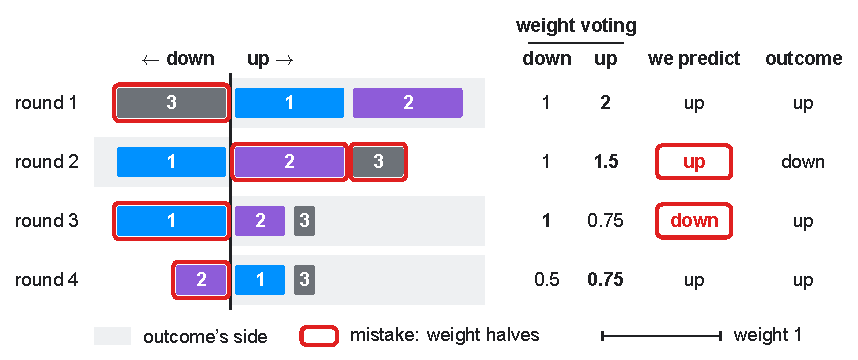
\includegraphics[width=\textwidth,height=0.65\paperheight,keepaspectratio]{assets/Fig-WMA-Weights.pdf}

  \vspace{0.2em}
  \raggedright
  Expert 1 made one mistake and experts 2 and 3 made two. We made two, so our
  regret against the best expert is
  $R_{\mathrm{WMA}}(4)=2-\min\{1,2,2\}=1$.
  \lecturesource{Weighted Majority Algorithm (WMA): Worked Example figure, caption, and regret.
    Figure: ../figs/Fig-WMA-Weights (TikZ, October 19, 2026).}
\end{frame}

\begin{frame}{Mistake Guarantee}
  Let $M_i^{(t)}$ be the mistakes of expert $i$ up to time $t$, and $M^{(t)}$
  our mistakes. For every expert $i$:
  \[
    \boxed{M^{(t)}\le\frac{2\ln n}{\epsilon}+2(1+\epsilon)\,M_i^{(t)}}
  \]

  \vspace{0.3em}
  \begin{itemize}\setlength{\itemsep}{0.6em}
    \item The guarantee is \hilite{multiplicative}: our mistakes are at most
      $2(1+\epsilon)$ times the best expert's, plus the constant
      $2\ln n/\epsilon$, which does not depend on the number of rounds.
    \item The algorithm is \hilite{deterministic}: the same predictions and
      outcomes always produce the same votes.
  \end{itemize}
  \lecturesource{Weighted Majority Algorithm (WMA): Mistake Guarantee theorem and the two features.}
\end{frame}

\begin{frame}{Why Choose an Expert at Random?}
  Because the vote is deterministic, an omniscient adversary can compute it and
  choose the opposite outcome. Suppose two experts always disagree:
  \begin{itemize}\setlength{\itemsep}{0.4em}
    \item The adversary makes us wrong in all $T$ rounds.
    \item In every round exactly one of the two experts is right, so the better
      expert makes at most $T/2$ mistakes.
  \end{itemize}

  \vspace{0.4em}
  No deterministic rule can guarantee fewer than \hilite{twice} the best
  expert's mistakes.

  \vspace{0.6em}
  Choosing an expert at random takes away this advantage. If the adversary
  fixes the outcomes before we draw, our expected cost exceeds the best
  expert's by at most a term that grows more slowly than the number of rounds,
  an \hilite{additive} guarantee.
  \lecturesource{Weighted Majority Algorithm (WMA): Mistake Guarantee, the "Why choose an expert at random?" paragraph and the additive-guarantee paragraph.}
\end{frame}

\begin{frame}{Multiplicative Weights: Problem Setting}
  We follow one expert chosen at random in proportion to its weight. The
  adversary fixes the advice and the outcomes in advance.

  \vspace{0.3em}
  \begin{itemize}\setlength{\itemsep}{0.3em}
    \item Sample an expert from our distribution over experts,
      $i\sim\texttt{Categorical}(\pv^{(t)})$, and follow its recommendation.
    \item Each expert's cost is $m_i^{(t)}\in[-1,1]$: $-1$ if correct and $+1$
      if incorrect. Together, they form the cost vector $\mv^{(t)}$.
  \end{itemize}
  The total expected cost and the \hilite{regret} against the
  \hilite{best expert in hindsight} are:
  \[
    L_A=\sum_{t=1}^{T}\sum_{i=1}^{n}p_i^{(t)}m_i^{(t)},
    \qquad
    R(T)=L_A-\min_{i}\sum_{t=1}^{T}m_i^{(t)}.
  \]
  A \hilite{sublinear} regret bound grows more slowly than $T$, so the bound on
  $R(T)/T$ vanishes as $T\to\infty$.
  \lecturesource{Multiplicative Weights Algorithm (MWA): opening paragraph and Problem Setting.}
\end{frame}

\begin{frame}{Multiplicative Weights: Pseudocode}
  \textbf{Initialize}: Given $n$ experts, the number of rounds $T\ge1$, and a
  learning rate $0<\eta\le1/2$, set $w_i^{(1)}\gets1$ for each expert $i$.

  \vspace{0.3em}
  For $t=1,2,\ldots,T$ \textbf{do}:
  \begin{enumerate}\setlength{\itemsep}{0.3em}
    \item Ask each expert $i$ for its answer $\hat y_i^{(t)}$. Choose expert $i$
      with probability $p_i^{(t)}=w_i^{(t)}/\sum_{j=1}^{n}w_j^{(t)}$ and follow
      its answer.
    \item The adversary (nature) reveals $y_t$. Compute each expert's cost:
      $m_i^{(t)}=-1$ if $\hat y_i^{(t)}=y_t$, and $+1$ otherwise.
    \item Update the weight of each expert $i$:
      \[
        w_i^{(t+1)}\gets w_i^{(t)}\cdot\bigl(1-\eta\cdot m_i^{(t)}\bigr).
      \]
  \end{enumerate}

  \vspace{0.3em}
  The learning rate $\eta$ controls how quickly the weights shift toward the
  better experts.
  \lecturesource{Multiplicative Weights Algorithm (MWA): Algorithm and the paragraph after it. Preserve the Initialize/For/numbered-step format.}
\end{frame}

\begin{frame}{Regret Bound}
  For costs $m_i^{(t)}\in[-1,1]$ and $0<\eta\le1/2$, for any expert $i$:
  \[
    \sum_{t=1}^{T}\pv^{(t)}\cdot\mv^{(t)}
    \le\sum_{t=1}^{T}m_i^{(t)}+\eta\sum_{t=1}^{T}\bigl|m_i^{(t)}\bigr|+\frac{\ln n}{\eta}
    \quad\Longrightarrow\quad
    R(T)\le\eta T+\frac{\ln n}{\eta},
  \]
  taking $i$ to be the best expert and using $|m_i^{(t)}|\le1$.

  \vspace{0.3em}
  Choosing $\eta=\sqrt{\ln n/T}$, which satisfies $\eta\le1/2$ when
  $T\ge4\ln n$:
  \[
    \boxed{R(T)\le2\sqrt{T\ln n}}
  \]
  The average regret per round is at most $2\sqrt{\ln n/T}$, which vanishes as
  $T\to\infty$: MWA does nearly as well as the best expert.
  \lecturesource{Multiplicative Weights Algorithm (MWA): Theoretical Regret Bound.}
\end{frame}

\begin{frame}{Compare the Two Guarantees}
  Both algorithms use \hilite{full feedback}: we score and update every expert.

  \vspace{0.4em}
  \centering
  {\small\setlength{\tabcolsep}{5pt}%
  \begin{tabular}{>{\raggedright\arraybackslash}p{0.2\textwidth}>{\raggedright\arraybackslash}p{0.3\textwidth}>{\raggedright\arraybackslash}p{0.38\textwidth}}
    \toprule
    \textbf{Algorithm} & \textbf{Prediction rule} & \textbf{Guarantee}\\
    \midrule
    Weighted majority & Weighted binary vote & Mistakes at most $2(1+\epsilon)$ times the best expert's, plus $2\ln n/\epsilon$\\
    \addlinespace
    Multiplicative weights & Sample an expert by weight & Expected cost at most $2\sqrt{T\ln n}$ above the best expert's, with $\eta=\sqrt{\ln n/T}$ and $T\ge4\ln n$\\
    \bottomrule
  \end{tabular}}

  \vspace{0.6em}
  \raggedright
  With $\ell_i^{(t)}=1$ for a mistake and $0$ otherwise, the signed cost is
  $m_i^{(t)}=2\ell_i^{(t)}-1$. The signed-cost regret is twice the expected
  mistake regret, so in mistakes the bound is $\sqrt{T\ln n}$.
  \lecturesource{Multiplicative Weights Algorithm (MWA): Compare the Two Guarantees table and the loss-convention paragraph.}
\end{frame}

\begin{frame}{Lab: Weighted Majority on the Stock Market}
  In the \href{\lablink}{lab}, we implement the weighted majority algorithm
  and use it to combine the advice of several experts:

  \vspace{0.6em}
  \begin{itemize}\setlength{\itemsep}{0.6em}
    \item each expert is a ticker, such as QQQ or AAPL, predicting whether the
      \hilite{SPY} exchange-traded fund goes up or down each trading day,
    \item we check the \hilite{mistake bound}, first when the experts see the
      same day's price moves and then when they must \hilite{forecast} the next
      day.
  \end{itemize}
  \slidenote{Lab:}{\href{\lablink}{The weighted majority algorithm on the stock market}}
  \lecturesource{Lab section. Lab notebook: introduction and Learning Objectives.}
\end{frame}

\begin{frame}{Summary}
  We introduced online learning and two algorithms that learn from expert
  advice.

  \vspace{0.5em}
  {\large\textbf{\ink{Key takeaways}}}
  \vspace{0.3em}
  \begin{itemize}\setlength{\itemsep}{0.6em}
    \item \textbf{\ink{Online learning and regret.}} We measured an algorithm in
      a repeated game by its regret against the best fixed strategy in hindsight.
    \item \textbf{\ink{The weighted majority algorithm.}} A weighted vote bounds
      our mistakes by two to three times the best expert's, plus a constant.
    \item \textbf{\ink{The multiplicative weights algorithm.}} Following an expert
      drawn by weight gives a regret bound that grows with the square root of
      the number of rounds.
  \end{itemize}

  \vspace{0.5em}
  Both algorithms rely on full feedback: once the outcome is revealed, we can
  score every expert.
  \lecturesource{Summary: three key takeaways and concluding sentence.}
\end{frame}

\end{document}
